
\subsection{Evaluation with Synthetically Injected Errors}
Here we experiment on data sets where we synthetically inject errors of three kinds - insertion, deletion, and substitution. The real data sets used in our evaluation in Section \ref{sec:evaluation-real} belonged to Illumina and therefore had primarily substitution errors (about 99\% of all errors). Hence our synthetic injections are meant to uncover if the relationship between perplexity and error rate holds for the other error types. 
We start by randomly collecting 100K short reads from the reference genome (\ie, without any error) for each of the two organisms used in the real data sets---\textit{E. coli} (D1, D2) and \textit{Acinetobacter} (D3). Afterward, we inject errors of each type as follows:
\begin{enumerate}[leftmargin=*]
\item \textbf{Deletion:} We select the index of injection (position from which to delete sequence), which follows a uniform distribution U(0,$l-d$), where $l$ is the length of the read and $d$ is the length to delete.
\item \textbf{Insertion:} Similar to deletion errors, the index of insertion follows a uniform distribution U(0,$l-I$), where $l$ is the length of the read and $I$ is the length of inserted segment. Moreover, each base pair in the inserted segment follows a uniform distribution over the four base pairs (A, C, G, or T).
\item \textbf{Substitution:} For this type of synthetic errors, we select $k$ positions of substitutions following a uniform distribution U(0,$l$), where $l$ denotes the length of the read. Second, we substitute each base pair of the $k$ positions with another base pair following a uniform distribution over the four base pairs (A, C, G, or T). Note that there is one-in-four chance that the substitution results in the same base pair. 
\end{enumerate}
We test the proposed approach against two levels of synthetic errors: low error rate (Uniform in (1, 5) bp in error per read), and high error rate (Uniform in (6, 10) bp in error per read). In all cases, the language model is trained using the original data set, mentioned in Table \ref{tbl:Datasets_Description}, with the natural ambient rate of error. 
Figure \ref{figure:Synthetic_Errors_Detection} shows the results for the perplexity metric in the data set {\em after} error injection (\ie, without doing correction), for the three error types and an equi-probable mixture of the three. The results show that for all types of errors, the direct quantitative relation between error rate and perplexity holds---the perplexity values are higher for high error rate injection. One observation is that the values of perplexity for insertion and substitution errors are higher than for deletion errors. For example, insertion and substitution perplexities are 3X \& 4.7X the deletion perplexity for high error rate data sets, and 2X \& 1.5X for low error rate data sets. This is expected because in deletion errors, the segment of the read after the index of deletion is a correct segment and hence is expected by the language model. On the other hand, for insertion and substitutions, the added synthetic base pairs will most likely construct wrong segments. Such segments will have very low counts in the language model and therefore produce higher overall perplexities.
Another observation is that the perplexities for the injection into data set D1 are higher than for D3. This is likely because D3 had a higher natural ambient rate of error and hence the additional injection does not cause as much increase in the perplexity metric.

\begin{figure}[t] \label{figure:Synthetic_Errors_Detection}
%\centering
\begin{minipage}[t]{1.0\textwidth}
\begin{minipage}[t]{.24\textwidth}
\centering
  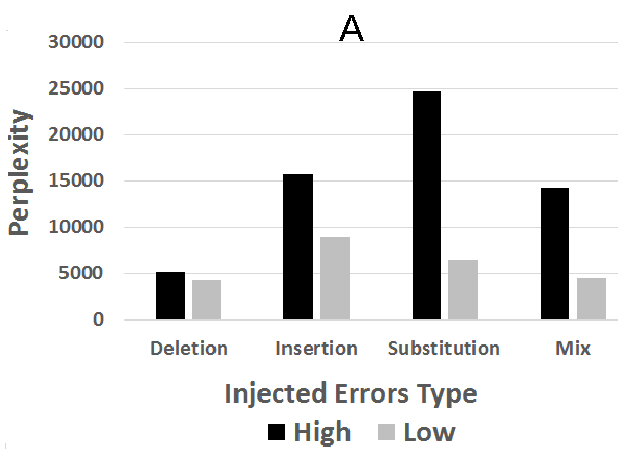
\includegraphics[width=\linewidth]{figs/Synth_NG_12.pdf}
 % \caption{A}
\end{minipage}%
\begin{minipage}[t]{.24\textwidth}
\centering
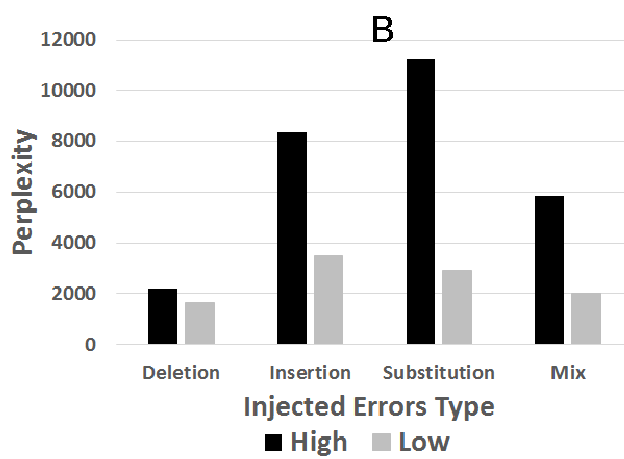
\includegraphics[width=\linewidth]{figs/Synth_NG_3.pdf}
 % \caption{B}
\end{minipage}%
\begin{minipage}[t]{.24\textwidth}
\centering
  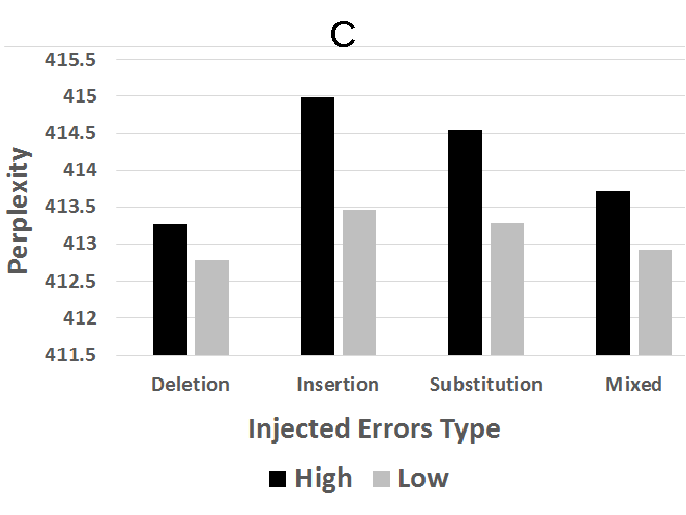
\includegraphics[width=\linewidth]{figs/Synth_RNN_12.pdf}
 % \caption{C}
\end{minipage}
\begin{minipage}[t]{.24\textwidth}
\centering
  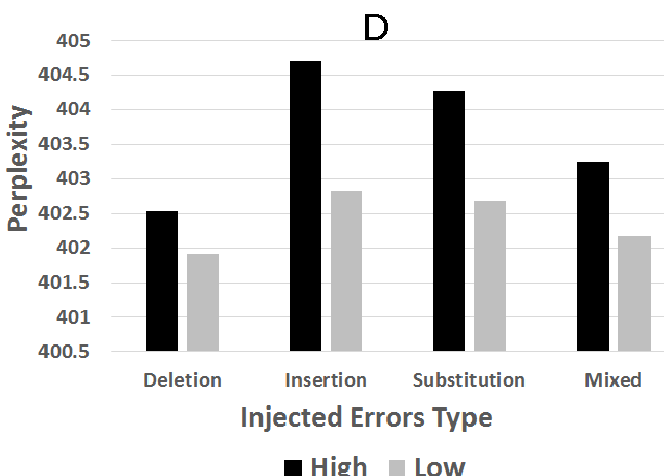
\includegraphics[width=\linewidth]{figs/Synth_RNN_3.pdf}
  %\caption{D}
\end{minipage}
\end{minipage}
  \caption{N-Gram (Figures A and B) and RNN (Figures C and D)  Perplexity metric for different types of synthetic errors: Indels and Substitution errors, and a mixture of the three for \textit{E. coli} str reference genome (Figures A and C) and \textit{Acinetobacter} sp. reference genome (Figures B and D). We compare two versions of such errors: high and low error rates.}
\label{figure:Synthetic_Errors_Detection}
\end{figure}

% \begin{figure}

% \end{figure}
% \begin{figure}
  
% \end{figure}
